% ===== 原文 pp.118–129（PDF p.133–144）=====
% 第 3 章 §3.4 末（pp.118–125）、§3.5（pp.126–128）、§3.6（p.129）
% tag 区间：3.6–3.9（(3.6)(3.7) 在 p.121；(3.8) 在 p.122；(3.9) 在 p.124）
% 本块不写章标题；§3.4 标题由 c03b 在 p.117 写出，本块从 p.117 末句“因此”之后续写，不重开小节。
% §3.5、§3.6 的小节标题由本块写出。
% [原文 p.118]
所有把恒等同态 $A[t]/(t^k)\to A[t]/(t^k)$ 提升为 $A[t]/(t^{k+1})\to A[t]/(t^{k+1})$ 的可能提升，被典范地等同于 $\Gamma(X,\Theta_{X/k})$。

选定一组提升 $\theta_{ij}^{k}$ 之后，我们现在要在 $U_{ij\ell}$ 上施加条件
\[
  \theta_{j\ell}^{k}\circ\theta_{ij}^{k}=\theta_{i\ell}^{k},
\]
以便这些态射诱导相容的粘合。当然，
\[
  \theta_{j\ell}^{k}\circ\theta_{ij}^{k}\circ(\theta_{i\ell}^{k})^{-1}\equiv\mathrm{id}\pmod{t^k}.
\]
于是 $U_{ij\ell}\times\mathcal{O}_k$ 的这个自同构 $\theta_{j\ell}^{k}\circ\theta_{ij}^{k}\circ(\theta_{i\ell}^{k})^{-1}$ 是恒等的提升，从而由某个元素 $\psi_{ij\ell}\in\Gamma(U_{ij\ell},\Theta_{X/k})$ 决定。当然 $(U_{ij\ell},\psi_{ij\ell})$ 是一个 Čech 2-余循环，它定义了元素 $\operatorname{ob}(X_{k-1}/\mathcal{O}_{k-1})\in H^2(X,\Theta_{X/k})$。

这个元素恰是把 $X_{k-1}$ 提升为 $X_k$ 的障碍。事实上，该上同调类为零当且仅当存在 $\Theta_{X/k}$ 的 Čech 余链 $(U_{ij},\psi_{ij})$，使得 $\psi_{ij}+\psi_{j\ell}-\psi_{i\ell}=\psi_{ijk}$。于是，若我们把最初选定的提升 $\theta_{ij}^{k}$ 用从 $(\theta_{ij}^{k})^{*}$ 减去 $t^k\psi_{ij}$ 的办法作修改，便可把 $\psi_{ij\ell}$ 换成 $\psi_{ij\ell}-(\psi_{ij}+\psi_{j\ell}-\psi_{j\ell})=0$。这样在新的选法下，$\theta_{j\ell}^{k}\circ\theta_{ij}^{k}=\theta_{i\ell}^{k}$，并且开集 $U_i\times\mathcal{O}_k$ 可以粘合。反之，若能找到可粘合的提升 $\theta_{ij}^{k}$，则 2-余循环 $\operatorname{ob}(X_{k-1}/\mathcal{O}_{k-1})$ 显然在 $H^2(X,\Theta_{X/k})$ 中消失。

% [Tutor Note: 原文 p.118 此处有两处印刷笔误（照排并在此注明正确形式）：①Čech 余链的条件应作 $\psi_{ij}+\psi_{j\ell}-\psi_{i\ell}=\psi_{ij\ell}$，原文右端印作 $\psi_{ijk}$；②下一句中被减去的项应作 $(\psi_{ij}+\psi_{j\ell}-\psi_{i\ell})$，原文末项印作 $\psi_{j\ell}$。两处以余循环的支撑下标 $i,j,\ell$ 为准即可看出。]

此外，提升的选取是自由的。对 $\Theta_{X/k}$ 的任一 Čech 1-余循环 $(U_{ij},\psi_{ij})$，我们都可以把给定的一组提升 $\theta_{ij}^{k}$ 换成在 $(\theta_{ij}^{k})^{*}$ 上加上 $t^k\psi_{ij}$，而不影响粘合的相容性。

任何这样的提升选取都可以用某个 1-余链 $(U_i,\psi_i)$ 的 Čech 微分来修改，而这将给出同构的提升 $X_k$。这个同构经由等同 $U_i^k\to U_i^k$ 诱导，后者在模 $t^k$ 下是恒等，从而由导子 $t^k\psi_i$ 决定。

我们得出结论：$X_{k-1}\to\mathcal{O}_{k-1}$ 到 $X_k\to\mathcal{O}_k$ 的提升，在同构意义下，构成 $H^1(X,\Theta_{X/k})$ 上的一个挠子。

总之，以上论证概要地证明了

\begin{proposition}
给定非奇异分离簇 $X/k$，以及 $X/k$ 到平坦形变 $X_{k-1}/\mathcal{O}_{k-1}$ 的提升，则存在元素
\[
  \operatorname{ob}(X_{k-1}/\mathcal{O}_{k-1})\in H^2(X,\Theta_{X/k}),
\]
使得 $X_{k-1}/\mathcal{O}_{k-1}$ 能提升为 $X_k/\mathcal{O}_k$ 当且仅当 $\operatorname{ob}(X_{k-1}/\mathcal{O}_{k-1})=0$。此外，若 $X_{k-1}/\mathcal{O}_{k-1}$ 存在提升 $X_k/\mathcal{O}_k$，则所有这类提升的集合是 $H^1(X,\Theta_{X/k})$ 上的一个挠子。
\end{proposition}

这实际上只是形变理论的一个特例，更深入的研究还能说明更多东西。然而这个例子为我们所需的内容提供了一个很好的模型。

记住上述框架，我们来考虑对数版本。设有对数光滑态射 $X^{\dagger}\to\operatorname{Spec} k^{\dagger}$。我们想理解形如 $X_k^{\dagger}\to\mathcal{O}_k^{\dagger}$ 的对数光滑形变。

现在，使这一情形区别于上述通常情形的第一个问题是：$\mathcal{O}_k$ 上的对数结构的选取并不唯一。我们将限制为由图表 $\mathbb{N}\to R_k$ 定义的细对数结构，该图表与 $\mathbb{N}\to R_k\to k$ 的复合把 $0$ 送到 $1$、把 $\mathbb{N}$ 的其他元素都送到 $0$。于是 $\mathcal{O}_k$ 上诱导的对数结构限制到 $\operatorname{Spec} k$ 上就是 $\operatorname{Spec} k$ 上的标准对数结构。

% [原文 p.119]
第二个问题是：在对数光滑形变理论中，形变通常不是局部平凡的。例如，由 $t\mapsto xy$ 给出的映射 $\operatorname{Spec} k[x,y]\to\operatorname{Spec} k[t]$ 是奇异（但对数光滑）簇 $xy=0$ 的一个对数光滑形变；这当然不是局部平凡的。

然而要点在于：若我们想要 $X^{\dagger}\to\operatorname{Spec} k^{\dagger}$ 在 $\mathcal{O}_k^{\dagger}$ 上（对 $\mathcal{O}_k$ 上对数结构的某种选取）的一个对数光滑形变 $X_k^{\dagger}\to\mathcal{O}_k^{\dagger}$，那么该形变 $X_k^{\dagger}\to\mathcal{O}_k^{\dagger}$ 的局部结构完全由 $\mathcal{O}_k$ 上的对数结构决定。这来自下列命题，我们不加证明地叙述它。见 [65]，命题 3.14 或 [63]，命题 8.3。

\begin{proposition}
设 $X^{\dagger}\to\operatorname{Spec} k^{\dagger}$ 对数光滑，$X$ 仿射。给定 $\mathcal{O}_k$ 上的细对数结构 $\mathcal{O}_k^{\dagger}$，其到 $\mathcal{O}_0=\operatorname{Spec} k$ 的限制是标准对数点，则 $X^{\dagger}\to\operatorname{Spec} k^{\dagger}$ 的对数光滑提升 $X_k^{\dagger}\to\mathcal{O}_k^{\dagger}$ 在同构意义下唯一。
\end{proposition}

例如，若 $X=\operatorname{Spec} k\times_{\operatorname{Spec}\mathbb{Z}[\mathbb{N}]}\mathbb{Z}[P]$ 对某个幺半群同态 $\mathbb{N}\to P$ 成立，则取 $X_k=\mathcal{O}_k\times_{\operatorname{Spec}\mathbb{Z}[\mathbb{N}]}\operatorname{Spec}\mathbb{Z}[P]$，其中映射 $\mathcal{O}_k\to\operatorname{Spec}\mathbb{Z}[\mathbb{N}]$ 由定义 $\mathcal{O}_k$ 上对数结构的图表 $\mathbb{N}\to R_k$ 决定。比如，若这个图表是平凡的（把 $1$ 送到 $0$），则 $X_k$ 是 $X$ 的平凡形变；但若图表例如由 $1\mapsto t$ 给出，则 $X_k$ 是 $X$ 的 $k$ 阶光滑化。

% [Tutor Note: 原文 p.119 的"图表平凡（$1\mapsto0$）时 $X_k$ 是平凡形变、图表由 $1\mapsto t$ 给出时是 $k$ 阶光滑化"可作核对锚点：图表 $\mathbb{N}\to R_k$ 把生成元送到 $0$ 时，$\mathcal{O}_k\times_{\operatorname{Spec}\mathbb{Z}[\mathbb{N}]}\operatorname{Spec}\mathbb{Z}[P]\cong X\times_k\mathcal{O}_k$，确是平凡形变；送到 $t$ 时对数结构非平凡，沿 $t=0$ 的纤维被"磨光"为 $X_k$。]

我们现在可以像先前那样进行。设有对数光滑的 $X^{\dagger}\to\operatorname{Spec} k^{\dagger}$，以及在 $\mathcal{O}_{k-1}$、$\mathcal{O}_k$ 上分别给定的对数结构 $\mathcal{O}_{k-1}^{\dagger}$、$\mathcal{O}_k^{\dagger}$，其中 $\mathcal{O}_k^{\dagger}$ 限制到 $\mathcal{O}_{k-1}^{\dagger}$ 与 $\operatorname{Spec} k$ 上的标准对数结构。再设我们有 $X^{\dagger}\to\operatorname{Spec} k^{\dagger}$ 的对数光滑提升 $X_{k-1}^{\dagger}\to\mathcal{O}_{k-1}^{\dagger}$，并想把它提升为 $X_k^{\dagger}\to\mathcal{O}_k^{\dagger}$。

像先前一样，取 $X^{\dagger}$ 的开仿射覆盖 $\{U_i^{\dagger}\}$。由上述命题，每个 $U_i^{\dagger}\to\operatorname{Spec} k^{\dagger}$ 唯一地提升为 $(U_i^{k-1})^{\dagger}\to\mathcal{O}_{k-1}^{\dagger}$，于是 $X_{k-1}^{\dagger}$ 由对数概形 $(U_i^{k-1})^{\dagger}$ 通过 $\mathcal{O}_{k-1}^{\dagger}$ 上的对数自同构
\[
  \theta_{ij}^{k-1}:(U_{ij}^{k-1})^{\dagger}\to(U_{ij}^{k-1})^{\dagger}
\]
粘合而成。然后我们选取提升
\[
  \theta_{ij}^{k}:(U_{ij}^{k})^{\dagger}\to(U_{ij}^{k})^{\dagger}.
\]
这里 $(U_i^{k})^{\dagger}$ 又是 $(U_i^{k-1})^{\dagger}$ 到 $\mathcal{O}_k^{\dagger}$ 上对数光滑概形的唯一提升。接着我们应用下列命题：

\begin{proposition}
设 $X^{\dagger}\to\operatorname{Spec} k^{\dagger}$ 对数光滑且 $X$ 仿射，并设给定对数光滑的 $X_{k-1}^{\dagger}\to\mathcal{O}_{k-1}^{\dagger}$，它限制到 $X^{\dagger}\to\operatorname{Spec} k^{\dagger}$，且给定对数光滑提升 $X_k^{\dagger}\to\mathcal{O}_k^{\dagger}$。则：
\begin{enumerate}[label=(\arabic*)]
\item 给定 $\mathcal{O}_{k-1}^{\dagger}$ 上的对数自同构 $\theta_{k-1}:X_{k-1}^{\dagger}\to X_{k-1}^{\dagger}$，它在 $X^{\dagger}$ 上限制为恒等，则 $\theta_{k-1}$ 到 $\mathcal{O}_k^{\dagger}$ 上的对数自同构 $\theta_k:X_k^{\dagger}\to X_k^{\dagger}$ 的提升集合是 $\Gamma(X,\Theta_{X^{\dagger}/k^{\dagger}})$ 上的一个挠子。
\item 在 $X_{k-1}^{\dagger}$ 上限制为恒等的对数自同构 $\theta_k:X_k^{\dagger}\to X_k^{\dagger}$（在 $\mathcal{O}_k^{\dagger}$ 上）的集合，典范同构于 $\Gamma(X,\Theta_{X^{\dagger}/k^{\dagger}})$。
\end{enumerate}
\end{proposition}

\begin{proof}[证明]
我们先不加证明地指出：$\theta_{k-1}$ 总能提升为自同构 $\theta_k$。这来自对数光滑性的无穷小提升判据：见 [65]，命题 3.4 与推论 3.11，或 [63]，定理 4.1。

% [原文 p.120]
$X_k^{\dagger}$ 在 $\mathcal{O}_k^{\dagger}$ 上的对数自同构由 $R_k$-代数层的自同构
\[
  \theta_k^{*}:\mathcal{O}_{X_k}\to\mathcal{O}_{X_k}
\]
以及自同构
\[
  \theta_k^{\#}:\mathcal{M}_{X_k}\to\mathcal{M}_{X_k}
\]
诱导，后者与 $\theta_k^{*}$ 及 $\mathcal{O}_k^{\dagger}$ 上的对数结构相容。设有两个这样的自同构 $\theta_k$ 与 $\bar\theta_k$，它们限制到 $X_{k-1}^{\dagger}$ 的同一自同构 $\theta_{k-1}$。则在 $X_k$ 上如下定义一个取值于 $t^k\mathcal{O}_{X_k}=t^k\mathcal{O}_X$ 的对数导子 $(\mathrm{D},\mathrm{Dlog})$。对 $\mathcal{O}_{X_k}$ 的截面 $f$，定义
\[
  \mathrm{D}f=\bar\theta_k^{*}(f)-\theta_k^{*}(f)\in t^k\mathcal{O}_{X_k}=t^k\mathcal{O}_X.
\]
则 $\mathrm{D}$ 是通常导子：
\begin{align*}
  \mathrm{D}(f\cdot g)
  &=\bar\theta_k^{*}(f)\cdot\bar\theta_k^{*}(g)-\theta_k^{*}(f)\cdot\theta_k^{*}(g)\\
  &=\bar\theta_k^{*}(f)\cdot\bigl(\bar\theta_k^{*}(g)-\theta_k(g)\bigr)
    +\bigl(\bar\theta_k^{*}(f)-\theta_k^{*}(f)\bigr)\cdot\theta_k^{*}(g)\\
  &=f\mathrm{D}g+(\mathrm{D}f)g.
\end{align*}
这里第三个等号成立，是因为 $\mathrm{D}f$ 与 $\mathrm{D}g$ 落在 $t^k\mathcal{O}_{X_k}$ 中，而 $\theta_k^{*}$ 与 $\bar\theta_k^{*}$ 在模 $t$ 下是恒等。

下面如下定义 $\mathrm{Dlog}$。对 $m\in\mathcal{M}_{X_k}$，有 $\bar\theta_k^{\#}(m)\equiv\theta_k^{\#}(m)\pmod{t^k}$；又因 $\theta_k^{\#}$ 与 $\bar\theta_k^{\#}$ 在 $\overline{\mathcal{M}}_{X_k}=\overline{\mathcal{M}}_X$ 上诱导恒等，我们有
\[
  \bar\theta_k^{\#}(m)=h_m\cdot\theta_k^{\#}(m),
\]
其中 $h_m\in1+t^k\mathcal{O}_{X_k}$。定义 $\mathrm{Dlog}(m)=h_m-1$。于是 $(\mathrm{D},\mathrm{Dlog})$ 构成 $\mathcal{O}_k^{\dagger}$ 上的对数导子：我们有
\begin{align*}
  \mathrm{D}(\alpha_{X_k}(m))
  &=\bar\theta_k^{*}(\alpha_{X_k}(m))-\theta_k^{*}(\alpha_{X_k}(m))\\
  &=\alpha_{X_k}\bigl(\bar\theta_k^{\#}(m)\bigr)-\alpha_{X_k}\bigl(\theta_k^{\#}(m)\bigr)\\
  &=\alpha_{X_k}\bigl((1+\mathrm{Dlog}(m))\theta_k^{\#}(m)\bigr)-\alpha_{X_k}\bigl(\theta_k^{\#}(m)\bigr)\\
  &=\mathrm{Dlog}(m)\cdot\alpha_{X_k}\bigl(\theta_k^{\#}(m)\bigr)\\
  &=\mathrm{Dlog}(m)\cdot\alpha_{X_k}(m).
\end{align*}
最后一行同样是因为 $\mathrm{Dlog}(m)\in t^k\mathcal{O}_{X_k}$。此外，若 $\pi:X_k^{\dagger}\to\mathcal{O}_k^{\dagger}$ 是给定的态射，则 $\mathrm{Dlog}(\pi^{\#}(m))=0$，因为 $\bar\theta_k^{\#}(\pi^{\#}(m))=\pi^{\#}(m)=\theta_k^{\#}(\pi^{\#}(m))$——$\theta_k$ 与 $\bar\theta_k$ 都是 $\mathcal{O}_k^{\dagger}$ 上的自同构。

注意 $\mathrm{D}(f)$ 与 $\mathrm{Dlog}(m)$ 只依赖于 $f$ 与 $m$ 模 $t$。因此 $(\mathrm{D},\mathrm{Dlog})$ 可以看作 $\Gamma(X,\Theta_{X^{\dagger}/k^{\dagger}})$ 中的对数导子（更确切地说，是 $t^k\Gamma(X,\Theta_{X^{\dagger}/k^{\dagger}})$ 中的）。此外反过来，给定 $\theta_k$ 与 $(\mathrm{D},\mathrm{Dlog})$ 便决定了 $\bar\theta_k$。

这就给出 (1)。对 (2)，取 $\theta_k$ 为恒等，于是任一 $\bar\theta_k$ 由 $\Gamma(X,\Theta_{X^{\dagger}/k^{\dagger}})$ 中的导子典范决定。
\end{proof}

然后我们就可以沿用通常形变理论情形中所作的同样论证，得到：

% [原文 p.121]
\begin{proposition}
设有对数光滑态射 $X^{\dagger}\to\operatorname{Spec} k^{\dagger}$，其中 $X$ 在 $k$ 上分离，并且该态射提升为对数光滑态射 $X_{k-1}^{\dagger}\to\mathcal{O}_{k-1}^{\dagger}$（对 $\mathcal{O}_{k-1}$ 上对数结构的某种选取）。给定该对数结构到 $\mathcal{O}_k$ 的提升，则存在元素 $\operatorname{ob}(X_{k-1}^{\dagger}/\mathcal{O}_{k-1}^{\dagger})\in H^2(X,\Theta_{X^{\dagger}/k^{\dagger}})$，使得 $X_{k-1}^{\dagger}\to\mathcal{O}_{k-1}^{\dagger}$ 能提升为对数光滑态射 $X_k^{\dagger}\to\mathcal{O}_k^{\dagger}$ 当且仅当 $\operatorname{ob}(X_{k-1}^{\dagger}/\mathcal{O}_{k-1}^{\dagger})=0$。此外，这类提升在同构意义下的集合是 $H^1(X,\Theta_{X^{\dagger}/k^{\dagger}})$ 上的一个挠子。
\end{proposition}

应用这个命题的最理想情形是 $H^2(X,\Theta_{X^{\dagger}/k^{\dagger}})=0$，此时没有障碍。例如 $X$ 是曲线时就是这种情形。

为第 4 章的需要，我们将要考虑一个更复杂的形变理论问题。设 $X$ 是带标准对数结构（由 $\partial X\subseteq X$ 诱导）的环面簇，并带有由 $X$ 上的单项式函数诱导的态射 $\pi:X^{\dagger}\to(\mathbb{A}^1_k)^{\dagger}$。以下讨论中我们固定这些数据。再考虑对数光滑曲线 $C_0^{\dagger}\to\operatorname{Spec} k^{\dagger}=\mathcal{O}_0^{\dagger}$，并设给定交换图表
\begin{equation}
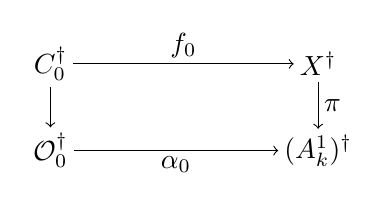
\begin{tikzpicture}[baseline=(current bounding box.center), every node/.style={inner sep=2pt}]
  \node (A) at (0,1.1) {$C_0^{\dagger}$};
  \node (B) at (3.4,1.1) {$X^{\dagger}$};
  \node (C) at (0,0) {$\mathcal{O}_0^{\dagger}$};
  \node (D) at (3.4,0) {$(\mathbb{A}^1_k)^{\dagger}$};
  \draw[->] (A) -- node[above] {$f_0$} (B);
  \draw[->] (A) -- (C);
  \draw[->] (B) -- node[right] {$\pi$} (D);
  \draw[->] (C) -- node[below] {$\alpha_0$} (D);
\end{tikzpicture} \tag{3.6}
\end{equation}
这里 $\alpha_0:\mathcal{O}_0\to\mathbb{A}^1_k$ 映到原点。我们想理解图表 (3.6) 到图表
\begin{equation}
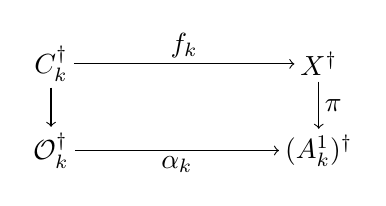
\begin{tikzpicture}[baseline=(current bounding box.center), every node/.style={inner sep=2pt}]
  \node (A) at (0,1.1) {$C_k^{\dagger}$};
  \node (B) at (3.4,1.1) {$X^{\dagger}$};
  \node (C) at (0,0) {$\mathcal{O}_k^{\dagger}$};
  \node (D) at (3.4,0) {$(\mathbb{A}^1_k)^{\dagger}$};
  \draw[->] (A) -- node[above] {$f_k$} (B);
  \draw[->] (A) -- (C);
  \draw[->] (B) -- node[right] {$\pi$} (D);
  \draw[->] (C) -- node[below] {$\alpha_k$} (D);
\end{tikzpicture} \tag{3.7}
\end{equation}
的提升，其中底部水平箭头决定 $\mathcal{O}_k$ 上的对数结构：确实，给出态射 $\alpha_k:\mathcal{O}_k\to\mathbb{A}^1_k$ 与给出映射 $\mathbb{N}\to R_k$ 是同一回事，而后者给出 $\mathcal{O}_k$ 上对数结构的图表。

% [Tutor Note: 图表 (3.6)、(3.7) 原文的编号印在图的左侧空白处；本译按全稿规则把 \tag 放在显示公式处（图右侧）。另外注意 $\alpha_k:\mathcal{O}_k\to\mathbb{A}^1_k$ 这一支正是"对数结构的选择"之所在：它等同于图表 $\mathbb{N}\to R_k$，故 $\mathcal{O}_k$ 的对数结构随 $\alpha_k$ 而变，这解释了为何命题 3.40 要先固定对数结构再谈提升。]

我们把图表 (3.7) 的数据记作 $[f_k:C_k/\mathcal{O}_k\to X]$。

\begin{theorem}
设 $C_0$ 有理。考虑与微分层函子态射
\[
  f_0^{*}:f_0^{*}\Omega^1_{X^{\dagger}/(\mathbb{A}^1)^{\dagger}}\to\Omega^1_{C_0^{\dagger}/k^{\dagger}}
\]
对偶的映射
\[
  f_{0*}:\Theta_{C_0^{\dagger}/k^{\dagger}}\to f_0^{*}\Theta_{X^{\dagger}/(\mathbb{A}^1)^{\dagger}}.
\]
设 $f_{0*}$ 是单射，其余核记为 $\mathcal{N}_{f_0}$，称为 $f_0$ 的对数正规层。设
\[
  [f_{k-1}:C_{k-1}/\mathcal{O}_{k-1}\to X]
\]
是
\[
  [f_0:C_0/\mathcal{O}_0\to X]
\]
的提升。

% [原文 p.122]
则限制到 $[f_{k-1}:C_{k-1}/\mathcal{O}_{k-1}\to X]$ 的形如 $[f_k:C_k/\mathcal{O}_k\to X]$ 的提升的同构类集合，是 $H^0(C_0,\mathcal{N}_{f_0})$ 上的一个挠子。
\end{theorem}

\begin{proof}[证明]
首先注意，由于 $C_0$ 是曲线，$H^2(C_0,\Theta_{C_0^{\dagger}/k^{\dagger}})=0$，所以把 $C_{k-1}^{\dagger}\to\mathcal{O}_{k-1}^{\dagger}$ 提升为 $C_k^{\dagger}\to\mathcal{O}_k^{\dagger}$ 没有障碍。这类提升的集合构成 $H^1(C_0,\Theta_{C_0^{\dagger}/k^{\dagger}})$ 上的一个挠子。选定一个这样的提升。像上面那样，用仿射开集 $U_i$ 覆盖 $C_0$，其唯一加厚 $(U_i^{k-1})^{\dagger}$、$(U_i^{k})^{\dagger}$ 分别由 $\mathcal{O}_{k-1}^{\dagger}$ 与 $\mathcal{O}_k^{\dagger}$ 决定。我们有粘合映射
\begin{gather}
  \theta_{ij}^{k-1}:(U_{ij}^{k-1})^{\dagger}\to(U_{ij}^{k-1})^{\dagger}\notag\\
  \theta_{ij}^{k}:(U_{ij}^{k})^{\dagger}\to(U_{ij}^{k})^{\dagger}, \tag{3.8}
\end{gather}
满足 $\theta_{ij}^{k-1}=\theta_{ij}^{k}\pmod{t^k}$。我们还有由 $f_{k-1}$ 决定的映射 $f_i^{k-1}:(U_i^{k-1})^{\dagger}\to X^{\dagger}$；它们在 $U_{ij}^{k-1}$ 上必须满足相容性：
\[
  f_i^{k-1}=f_j^{k-1}\circ\theta_{ij}^{k-1}.
\]

按照形变理论的惯例，我们先选取 $f_i^{k-1}$ 的提升 $f_i^{k}:(U_i^{k})^{\dagger}\to X^{\dagger}$。这样的提升存在，实际上就是对数光滑性的无穷小提升判据：见 [65]，命题 3.4，或 [63]，定理 4.1。我们再次不加证明地陈述这一点。

提升 $f_i^{k}$ 的选取集合实际上是 $H^0(U_i,f_0^{*}\Theta_{X^{\dagger}/(\mathbb{A}^1)^{\dagger}})$ 上的一个挠子（见 [65]，命题 3.9）。确实，给出 $f_0^{*}\Theta_{X^{\dagger}/(\mathbb{A}^1)^{\dagger}}$ 的一个截面，等同于给出 $X$ 上取值于 $f_{0*}\mathcal{O}_{C_0}$ 的一个对数导子。现在给定 $f_i^{k-1}$ 的两个提升 $f_i^{k}$ 与 $\bar f_i^{k}$，我们由
\[
  \mathrm{D}g=(\bar f_i^{k})^{*}(g)-(f_i^{k})^{*}(g)
\]
（对 $X$ 上的函数 $g$）以及 $\mathrm{Dlog}(m)=h_m-1$（对 $\mathcal{M}_X$ 的截面 $m$）得到这样一个导子，其中 $h_m\in\mathcal{O}_{U_i^{k}}^{\times}$ 由
\[
  (\bar f_i^{k})^{\#}(m)=h_m(f_i^{k})^{\#}(m)
\]
定义。

这正像命题 3.39 的证明中那样是对数导子，并且在 $\mathbb{A}^1$ 上函数的拉回上为零，从而给出 $X^{\dagger}/(\mathbb{A}^1)^{\dagger}$ 的、取值于 $t^k\mathcal{O}_{U_i^{k}}\cong\mathcal{O}_{U_i}$ 的对数导子。于是它是 $\Gamma(U_i,f_0^{*}\Theta_{X^{\dagger}/(\mathbb{A}^1)^{\dagger}})$ 中的一个元素。反之，给定 $f_i^{k}$ 与这样的对数导子 $(\mathrm{D},\mathrm{Dlog})$，显然决定了 $\bar f_i^{k}$。若记 $(\mathrm{D},\mathrm{Dlog})=:\psi_i$，我们写
\[
  \bar f_i^{k}=f_i^{k}+t^k\psi_i.
\]

一旦选定了 $f_i^{k-1}$ 的提升 $f_i^{k}$，我们就可以对每个 $i,j$ 在 $U_{ij}^{k}$ 上比较 $f_i^{k}$ 与 $f_j^{k}\circ\theta_{ij}^{k}$。它们是同一个映射 $f_i^{k-1}=f_j^{k-1}\circ\theta_{ij}^{k-1}$ 的两个不同提升，因而相差一个元素 $\psi_{ij}\in\Gamma(U_{ij},f_0^{*}\Theta_{X^{\dagger}/(\mathbb{A}^1)^{\dagger}})$。这些给出 $C_0$ 上 $f_0^{*}\Theta_{X^{\dagger}/(\mathbb{A}^1)^{\dagger}}$ 的一个 Čech 1-余循环。然而，由例 3.32 (2)，$\Theta_{X^{\dagger}/(\mathbb{A}^1)^{\dagger}}$ 是平凡向量丛，因为 $X$ 是环面簇。又因 $C_0$ 假定有理，$H^1(C_0,f_0^{*}\Theta_{X^{\dagger}/(\mathbb{A}^1)^{\dagger}})=0$。于是提升没有障碍，我们得到提升 $[f_k:C_k/\mathcal{O}_k\to X]$。剩下的只是把这类提升的所有选取在同构意义下分类。

% [原文 p.123]
于是考虑数据 $\theta_{ij}^{k-1}$、$f_i^{k-1}$ 的两组提升，分别由 $\theta_{ij}^{k}$、$f_{ij}^{k}$ 与 $\bar\theta_{ij}^{k}$、$\bar f_{ij}^{k}$ 给出。那么 $\bar\theta_{ij}^{k}$ 与 $\theta_{ij}^{k}$ 相差某个 $t^k\psi_{ij}$，其中 $\psi_{ij}\in H^0(U_{ij},\Theta_{C_0^{\dagger}/k^{\dagger}})$；而 $\bar f_i^{k}$ 与 $f_i^{k}$ 相差 $t^k\eta_i$，其中 $\eta_i\in H^0(U_i,f_0^{*}\Theta_{X^{\dagger}/(\mathbb{A}^1)^{\dagger}})$。相容性条件
\[
  \bar f_i^{k}=\bar f_j^{k}\circ\bar\theta_{ij}^{k}
\]
变为
\[
  f_i^{k}+t^k\eta_i=f_j^{k}\circ\theta_{ij}^{k}+(f_{0*}(\psi_{ij})+\eta_j)t^k.
\]
于是 $\eta_i=f_{0*}(\psi_{ij})+\eta_j$，所以数据 $(\eta_i)_i$ 决定了 $\mathcal{N}_{f_0}$ 的一个截面。

反之，给定由 $(\bar\eta_i)_i$、$\bar\eta_i\in\Gamma(U_i,\mathcal{N}_{f_0})$ 决定的 $\mathcal{N}_{f_0}$ 的截面，我们可以把它们提升为 $\eta_i\in\Gamma(U_i,f_0^{*}\Theta_{X^{\dagger}/(\mathbb{A}^1)^{\dagger}})$，其中对某个 $\psi_{ij}$ 有 $\eta_i-\eta_j=f_{0*}(\psi_{ij})$。由于 $f_{0*}$ 假定为单射，这决定了 $\psi_{ij}$，从而由 $\theta_{ij}^{k}$、$f_i^{k}$ 决定了 $\bar\theta_{ij}^{k}$、$\bar f_i^{k}$。另一组提升 $(\eta_i')$ 会把 Čech 1-余循环 $\{(U_{ij},\psi_{ij})\}$ 改变一个上边缘，从而决定同构的提升。因此所有可能提升的集合是 $H^0(C_0,\mathcal{N}_{f_0})$ 上的一个挠子。
\end{proof}

为下一章的需要，我们还需要更多的装饰，如下。我们希望给 $C_0$ 作标记，考虑点 $x_1^0,\dots,x_s^0\in C_0$，把它们看作 $C_0\to\mathcal{O}_0$ 的截面 $x_i^0:\mathcal{O}_0\to C_0$。我们考虑提升 $[f_k:C_k/\mathcal{O}_k\to X]$ 以及 $C_k\to\mathcal{O}_k$ 的提升 $x_i^k:\mathcal{O}_k\to C_k$（即提升 $x_i^0$）。我们把这样一个提升的数据写作 $[f_k:C_k/\mathcal{O}_k\to X,\mathbf{x}^k]$。

\begin{theorem}
给定 $[f_0:C_0/\mathcal{O}_0\to X,\mathbf{x}^0]$，使得点 $x_1^0,\dots,x_s^0\in C_0^{\dagger}$ 都是对数光滑点，$C_0$ 有理，且 $f_{0*}$ 如定理 3.41 中那样是单射；定义 $\mathcal{N}_{f_0,\mathbf{x}^0}$ 为复合
\[
  \Theta_{C_0^{\dagger}/k^{\dagger}}\Bigl(-\sum_{i=1}^{s}x_i^0\Bigr)
  \hookrightarrow\Theta_{C_0^{\dagger}/k^{\dagger}}
  \xrightarrow{\ f_{0*}\ }f_0^{*}\Theta_{X^{\dagger}/(\mathbb{A}^1)^{\dagger}}
\]
的余核。给定提升
\[
  [f_{k-1}:C_{k-1}/\mathcal{O}_{k-1}\to X,\mathbf{x}^{k-1}],
\]
则
\[
  [f_k:C_k/\mathcal{O}_k\to X,\mathbf{x}^k]
\]
作为
\[
  [f_{k-1}:C_{k-1}/\mathcal{O}_{k-1}\to X,\mathbf{x}^{k-1}]
\]
的提升的集合，是 $H^0(C_0,\mathcal{N}_{f_0,\mathbf{x}^0})$ 上的一个挠子。
\end{theorem}

% [Tutor Note: 定理 3.42 的 $\mathcal{N}_{f_0,\mathbf{x}^0}$ 与定理 3.41 的 $\mathcal{N}_{f_0}$ 只差把 $\Theta_{C_0^{\dagger}/k^{\dagger}}$ 换成扭层 $\Theta_{C_0^{\dagger}/k^{\dagger}}(-\sum x_i^0)$：前者允许截面在标记点 $x_i^0$ 处取非零值，因而 $H^0(C_0,\mathcal{N}_{f_0,\mathbf{x}^0})$ 描述"可移动标记点"的形变。这正是定理 3.43 中映射 $\Xi$ 的定义域：提升存在归结为 $\Xi$ 满射，而提升集合是 $\ker\Xi$ 上的挠子。]

\begin{proof}[证明]
我们只需对定理 3.41 的论证作修改，把附加数据考虑进来。先不考虑映射 $f_0$，来理解提升 $C_k/\mathcal{O}_k,\mathbf{x}^k$。固定某个提升 $C_k^{\dagger}\to\mathcal{O}_k^{\dagger}$（它提升 $C_{k-1}^{\dagger}\to\mathcal{O}_{k-1}^{\dagger}$）。现在 $x_i^{k-1}:\mathcal{O}_{k-1}\to C_{k-1}$ 的提升 $x_i^k:\mathcal{O}_k\to C_k$ 的集合，实际上是 $C_0$ 在 $x_i^0$ 处的 Zariski 切空间上的一个挠子。确实，首先提升是存在的，因为 $C_k\to\mathcal{O}_k$ 在 $x_i^0$ 处光滑。（这是光滑态射的标准事实：它不过是光滑性的形式提升判据；例如见 [53]，§17。）其次，给定 $x_i^{k-1}$ 的两个提升 $x_i^k$、$\bar x_i^k$ 以及 $g\in\mathfrak{m}_{C_k,x_i^0}$（$\mathcal{O}_{C_k,x_i^0}$ 的极大理想），我们有
\[
  (\bar x_i^{k})^{*}(g)-(x_j^{k})^{*}(g)\in(t^k)\subseteq R_k.
\]
% [Tutor Note: 上式中的 $x_j$ 应为 $x_i$ 的笔误（原文 p.123 末，跨到 p.124）：左边比较的是同一个提升的两个版本在 $g$ 上的取值之差，下标须一致；由紧接的"诱导线性泛函 $\mathfrak{m}_{C_k,x_i^0}\to t^kk$"也可反推。本译照原文抄录并在此注明。]

% [原文 p.124]
这诱导出一个线性泛函 $\mathfrak{m}_{C_k,x_i^0}\to t^kk$，它显然下降给出线性泛函 $\mathfrak{m}_{C_0,x_i^0}/\mathfrak{m}_{C_0,x_i^0}^2\to t^kk$。这是 $C_0$ 在 $x_i^0$ 处的 Zariski 切空间的一个元素。反之，给定这样的线性函数，我们可以修改 $(x_j^{k})^{*}$ 得到 $(\bar x_i^{k})^{*}$。

注意，由于 $x_i^0$ 总是对数光滑点，事实上向量丛 $\Theta_{C_0^{\dagger}/k^{\dagger}}$ 与 $\Theta_{C_0/k}$ 在 $x_i^0$ 处的纤维一致，且两个纤维都与 $C_0$ 在 $x_i^0$ 处的 Zariski 切空间相同。

设有 $\mathcal{O}_k^{\dagger}$ 上的对数自同构 $\psi:C_k^{\dagger}\to C_k^{\dagger}$，它在模 $t^k$ 下是恒等，从而由 $\psi\in\Gamma(C_0,\Theta_{C_0^{\dagger}/k^{\dagger}})$ 诱导。再设给定 $x_i^{k-1}$ 的提升 $x_i^k:\mathcal{O}_k\to C_k$，并令
\[
  \bar x_i^k=\psi\circ x_i^k.
\]
那么 $\bar x_i^k$ 与 $x_i^k$ 之差就是 $\psi$ 在 $C_0$ 于 $x_i^0$ 处的 Zariski 切空间中的像。

这可总结为正合列
\begin{equation}
0\to\Theta_{C_0^{\dagger}/k^{\dagger}}(-\mathbf{x}^0)\to\Theta_{C_0^{\dagger}/k^{\dagger}}\to\bigoplus_{\ell=1}^{s}\Theta_{C_0^{\dagger}/k^{\dagger}}\otimes k(x_\ell^0)\to0. \tag{3.9}
\end{equation}
这里 $\Theta_{C_0^{\dagger}/k^{\dagger}}(-\mathbf{x}^0)$ 表示 $\Theta_{C_0^{\dagger}/k^{\dagger}}$ 用线丛
\[
  \mathcal{O}_{C_0}\Bigl(-\sum_{\ell=1}^{s}x_\ell^0\Bigr)
\]
扭一下所得的层，而 $k(x_\ell^0)$ 表示 $C_0$ 在 $x_\ell^0$ 处的剩余域。取 $C_0$ 的开仿射集 $U$ 上的截面，并带有诱导的加厚 $(U^{k-1})^{\dagger}$、$(U^{k})^{\dagger}$，则把映射 $\{x_\ell^{k-1}\mid x_\ell^0\in U\}$ 提升为映射 $x_\ell^{k}$（$x_\ell^0\in U$）的空间是
\[
  \Gamma\Bigl(U,\bigoplus_{\ell=1}^{s}\Theta_{C_0^{\dagger}/k^{\dagger}}\otimes k(x_\ell^0)\Bigr)
\]
上的一个挠子。

把 $(U^{k-1})^{\dagger}$ 的自同构提升为 $(U^{k})^{\dagger}$ 的自同构的集合是 $\Gamma(U,\Theta_{C_0^{\dagger}/k^{\dagger}})$ 上的一个挠子；而在所有满足 $x_\ell^0\in U$ 的 $\ell$ 上保持给定的 $x_\ell^{k-1}$ 的提升 $x_\ell^{k}$ 不变的那类提升，是 $\Gamma(U,\Theta_{C_0^{\dagger}/k^{\dagger}}(-\mathbf{x}^0))$ 上的一个挠子。

现在照例用仿射开子集 $(U_i^{k-1})^{\dagger}$ 覆盖 $C_{k-1}^{\dagger}$，并固定提升 $(U_i^{k})^{\dagger}$。对每个 $i$，设 $j_1,\dots,j_{s_i}$ 是使 $x_{j_\ell}^0\in U_i^{k-1}$（$1\le\ell\le s_i$）的指标。假设已有提升 $x_{j_\ell}^{k-1}:\mathcal{O}_{k-1}\to U_i^{k-1}$，我们可以把它们延拓为提升 $x_{j_\ell}^{k}:\mathcal{O}_k\to U_i^{k}$。另一方面，考虑由 (3.9) 给出的映射
\[
  \Psi_i:\Gamma(U_i,\Theta_{C_0^{\dagger}/k^{\dagger}})\to\bigoplus_{\ell=1}^{s_i}\Theta_{C_0^{\dagger}/k^{\dagger}}\otimes k(x_{j_\ell}^0).
\]
由于 $U_i$ 仿射，这个映射是满射。于是，模去 $(U_i^{k})^{\dagger}$ 的那些在模 $t^k$ 下为恒等的自同构，提升 $x_{j_\ell}^{k}$ 的选取是唯一的。

于是我们现在可以假定已固定开集 $(U_i^{k})^{\dagger}$ 与提升 $x_{j_\ell}^{k}:\mathcal{O}_k\to U_i^{k}$。我们只需把它们粘合起来。我们遵循通常的程序。不过，我们需要把那些落在 $U_{ij}^{k}$ 中的提升 $x_\ell^{k}$ 对应起来。按命题 3.40 中给出的通常

% [原文 p.125]
形变理论论证即可看出：$C_{k-1}/\mathcal{O}_{k-1},\mathbf{x}^{k-1}$ 的所有提升 $C_k/\mathcal{O}_k,\mathbf{x}^k$ 的集合构成
\[
  H^1(C_0,\Theta_{C_0^{\dagger}/k^{\dagger}}(-\mathbf{x}^0))
\]
上的一个挠子。

再重复定理 3.41 的论证，便得到所要的结果。
\end{proof}

最后的装饰如下。现在假设在上述数据之上，还给定 $\pi$ 的截面 $\sigma_1,\dots,\sigma_s:\mathbb{A}^1\to X$。假设我们从这样选取的 $[f_0:C_0/\mathcal{O}_0\to X,\mathbf{x}^0]$ 出发：$f_0(x_i^0)=\sigma_i(0)$（$1\le i\le s$）。换言之，我们对 $C_0$ 的标记点映到哪里施加了条件。注意我们也可以把这个条件写成 $f_0\circ x_i^0=\sigma_i\circ\alpha_0$。于是我们希望找到满足
\[
  f_k\circ x_i^k=\sigma_i\circ\alpha_k
\]
的提升 $[f_k:C_k/\mathcal{O}_k\to X,\mathbf{x}^k]$。（回忆 $\alpha_k:\mathcal{O}_k\to\mathbb{A}^1_k$ 是给定的映射。）

\begin{theorem}
设给定与定理 3.42 相同的假设，并附加假设 $f_0\circ x_i^0=\sigma_i\circ\alpha_0$（$1\le i\le s$）。用 $T_{X/\mathbb{A}^1,\sigma_i}$ 表示向量丛 $\Theta_{X^{\dagger}/(\mathbb{A}^1)^{\dagger}}$ 在 $\sigma_i(0)$ 处的纤维，等价地，表示向量丛 $f_0^{*}\Theta_{X^{\dagger}/(\mathbb{A}^1)^{\dagger}}$ 在 $x_i^0$ 处的纤维。它们可以写作 $\Theta_{X^{\dagger}/(\mathbb{A}^1)^{\dagger}}\otimes k(\sigma_i(0))$，或写作 $f_0^{*}(\Theta_{X^{\dagger}/(\mathbb{A}^1)^{\dagger}})\otimes k(x_i^0)$。则存在自然映射
\[
  \Xi:H^0(C_0,\mathcal{N}_{f_0,\mathbf{x}^0})\to\prod_{i=1}^{s}T_{X/\mathbb{A}^1,\sigma_i(0)}.
\]
映射 $H^0(C_0,\mathcal{N}_{f_0,\mathbf{x}^0})\to T_{X/\mathbb{A}^1,\sigma_i(0)}$ 由如下方式给出：把 $\mathcal{N}_{f_0,\mathbf{x}^0}$ 的一个截面在 $x_i^0$ 的邻域内局部提升为 $f_0^{*}\Theta_{X^{\dagger}/(\mathbb{A}^1)^{\dagger}}$ 的截面，再在 $x_i^0$ 处求值，得到 $T_{X/\mathbb{A}^1,\sigma_i(0)}$ 的元素。于是，给定
\[
  [f_0:C_0/\mathcal{O}_0\to X,\mathbf{x}^0]
\]
的提升
\[
  [f_{k-1}:C_{k-1}/\mathcal{O}_{k-1}\to X,\mathbf{x}^{k-1}]
\]
且满足 $f_{k-1}\circ x_i^{k-1}=\sigma_i\circ\alpha_{k-1}$（对所有 $i$），若 $\Xi$ 是满射，则存在
\[
  [f_{k-1}:C_{k-1}/\mathcal{O}_{k-1}\to X,\mathbf{x}^{k-1}]
\]
的提升
\[
  [f_k:C_k/\mathcal{O}_k\to X,\mathbf{x}^k]
\]
且满足 $f_k\circ x_i^k=\sigma_i\circ\alpha_k$（对所有 $i$）。此外，若提升存在，则这类提升的集合是 $\ker\Xi$ 上的一个挠子。
\end{theorem}

\begin{proof}[证明]
我们先说明 $\Xi$ 是良定义的。确实，$\mathcal{N}_{f_0,\mathbf{x}^0}$ 的截面 $s$ 的两个局部提升（提升为 $f_0^{*}\Theta_{X^{\dagger}/(\mathbb{A}^1)^{\dagger}}$ 的截面）相差一个在 $x_i^0$ 处消失的 $C_0$ 上的向量场。把 $f_{0*}$ 作用到这个向量场上，得到 $f_0^{*}\Theta_{X^{\dagger}/(\mathbb{A}^1)^{\dagger}}$ 的一个在 $x_i^0$ 处消失的截面，因此 $\Xi$ 是良定义的。

为得到结论，只需像通常那样考虑加厚 $(U_i^{k})^{\dagger}$，并固定映射 $x_\ell^{k}:\mathcal{O}_k\to U_i^{k}$（对各个 $\ell$）。所有可能的提升 $f_k,\mathbf{x}^k$ 都可通过修改 $(U_i^{k})^{\dagger}$ 的粘合以及修改映射 $f_k:(U_i^{k})^{\dagger}\to X$ 得到。注意粘合的修改不影响映射 $f_k\circ x_\ell^{k}$。所以，若把 $f_k:(U_i^{k})^{\dagger}\to X^{\dagger}$ 换成与 $f_k$ 相差一个 $f_0^{*}\Theta_{X^{\dagger}/(\mathbb{A}^1)^{\dagger}}$ 的截面 $\psi$ 的 $\bar f_k$，我们看到

% [原文 p.126]
对在 $\sigma_\ell(0)=f_0(x_\ell^0)$ 的邻域内定义的 $X$ 上的函数 $g$，
\begin{align*}
  (x_\ell^{k})^{*}\circ\bar f_k^{*}(g)
  &=(x_\ell^{k})^{*}\bigl(f_k^{*}(g)+t^k\psi(g)\bigr)\\
  &=(x_\ell^{k})^{*}\circ f_k^{*}(g)+t^k\psi(g)(x_\ell^0).
\end{align*}
于是这把 $(x_\ell^{k})^{*}\circ f_k^{*}$ 改变了 $T_{X/\mathbb{A}^1,x_\ell^0}$ 中由 $\psi$ 在 $x_\ell^0$ 处求值给出的元素。由于我们希望保证
\[
  (x_\ell^{k})^{*}\circ(f_k)^{*}=\alpha_k^{*}\circ\sigma_\ell^{*},
\]
而右端完全确定，结论便随之成立。
\end{proof}

\subsection{再论扭 de Rham 复形}

本节其实并不属于这里。它解释我们在 §2.2.1 中回避的一个技术要点：定理 2.31 只适用于 $W:X\to\mathbb{C}$ 是射影的情形。

由于对主要关注的例子——即 $\mathbb{P}^r$ 的镜像 Landau–Ginzburg 模型——并非如此，我们如下进行。若 $W:X\to\mathbb{C}$ 不是射影的、而只是拟射影的，则我们找到一个非奇异簇 $\overline{X}$ 使其包含 $X$，且 $D:=\overline{X}\setminus X$ 是正规交叉，并且 $W$ 延拓给出射影的 $W:\overline{X}\to\mathbb{C}$。然后我们考虑扭对数 de Rham 复形
\[
  \bigl(\Omega^{\bullet}_{\overline{X}}(\log D),d+dW\wedge\bigr),
\]
其中 $\Omega^p_{\overline{X}}(\log D)=\bigwedge^p\Omega^1_{\overline{X}}(\log D)$，而微分 $d+dW\wedge$ 一如先前由 $\omega\mapsto d\omega+dW\wedge\omega$ 给出。于是我们有（与定理 2.31 类似，由 Sabbah 在 [102] 中证明）

\begin{theorem}
在上述情形下，
\begin{align*}
  \mathbb{H}^i_{\mathrm{Zar}}\bigl(\overline{X},(\Omega^{\bullet}_{\overline{X}}(\log D),d+dW\wedge)\bigr)
  &\cong\mathbb{H}^i_{\mathrm{Zar}}\bigl(\overline{X},(\Omega^{\bullet}_{\overline{X}}(\log D),dW\wedge)\bigr)\\
  &\cong\mathbb{H}^i_{\mathrm{An}}\bigl(\overline{X},(\Omega^{\bullet}_{\overline{X}}(\log D),d+dW\wedge)\bigr).
\end{align*}
\end{theorem}

% [Tutor Note: 定理 3.44 是定理 2.31 在 $W$ 只拟射影时的替代版本（Sabbah [102]）：把 $X$ 紧化为 $\overline{X}$、取对数 de Rham 复形后，$\mathbb{H}^i_{\mathrm{Zar}}$ 与 $\mathbb{H}^i_{\mathrm{An}}$ 两种取法给出同一个群。注意 $\Omega^{\bullet}$ 的 $\bullet$ 表示全集次数（$\Omega^p=\bigwedge^p\Omega^1$），$\mathbb{H}$ 表示超上同调；这只在 $W$ 非真时才与定理 2.31 的结论形式不同。]

事实上，当 $W:X\to\mathbb{C}$ 不真时，应当使用的正确上同调群正是上述定理中出现的那些。

现在我们将对 $\mathbb{P}^r$ 的镜像施行这一程序。最终我们会看到所得答案与 §2.2.1 中的相同，所以这个计算可以放心跳过；但它确实很好地示范了环面技巧的运用。

照例令 $M=\mathbb{Z}^r$、$N=\operatorname{Hom}_{\mathbb{Z}}(M,\mathbb{Z})$ 等等，并令 $\Delta\subseteq N_{\mathbb{R}}$ 为由
\[
  \Delta:=\operatorname{Conv}(\{e_0,e_1,\dots,e_r\})
\]
给出的格多胞体，其中 $e_1,\dots,e_r$ 是 $N$ 的标准基，而
\[
  e_0=-\sum_{i=1}^{r}e_i.
\]
注意 $\Delta$ 实际上是自反多胞体（见例 1.28），其对偶为
\[
  \Delta^{*}:=\operatorname{Conv}\{e_0^{*},e_0^{*}+(r+1)e_1^{*},\dots,e_0^{*}+(r+1)e_r^{*}\},
\]
其中 $e_1^{*},\dots,e_r^{*}$ 是 $M$ 的对偶基，且
\[
  e_0^{*}=-\sum_{i=1}^{r}e_i^{*}.
\]

% [原文 p.127]
现在 $\Delta$ 定义了一个射影环面簇 $\mathbb{P}_{\Delta}$。我们定义 $X\cong(\mathbb{C}^{\times})^r$ 为 $\mathbb{P}_{\Delta}$ 的开环面轨道。我们把这里的 $X$ 与例 2.33 中所用的 $X$ 等同起来。在那个例子里，按现在的记号，我们取的是 $W=z^{e_1}+\cdots+z^{e_r}+\kappa z^{e_0}$。现在由注 3.5，任何 $n\in\Delta\cap N$ 都可以看作 $\mathcal{O}_{\mathbb{P}_{\Delta}}(1)$ 的一个截面。该线丛可以在 $\mathbb{P}_{\Delta}$ 的开环面轨道上平凡化，使得由 $n\in\Delta\cap N$ 决定的截面对应于 $X$ 上的正则函数 $z^n$。由于 $0\in\Delta$，这给出一个对应于 $X$ 上正则函数 $z^0=1$ 的截面。于是 $W$ 在 $X$ 上的表达式也可以写成
\[
  W=\frac{z^{e_1}+\cdots+z^{e_r}+\kappa z^{e_0}}{z^0},
\]
而把它写成这个比值后，它实际上延拓到 $\mathbb{P}_{\Delta}$ 上，成为 $\mathcal{O}_{\mathbb{P}_{\Delta}}(1)$ 的两个截面之比，从而定义了有理函数
\[
  W:\mathbb{P}_{\Delta}\dashrightarrow\mathbb{P}^1_k.
\]

现在有两个问题需要处理。第一，$\mathbb{P}_{\Delta}$ 相当奇异，这些奇点需要被消解。第二，$W$ 只是有理的，所以还需要进一步的爆破来消解 $W$ 的奇点。

为解决这些问题，我们先以环面方式消解 $\mathbb{P}_{\Delta}$ 的奇点。$\Delta$ 的法扇实际上正是由 $\Delta^{*}$ 的真面生成的锥的集合。为消解 $\mathbb{P}_{\Delta}$，我们可以通过选取 $\partial\Delta^{*}$ 的一个由标准单纯形构成的多面体分解 $\mathcal{P}$ 来加细法扇。于是由 $\mathcal{P}$ 的元素生成的锥构成的扇 $\Sigma$ 是 $\Delta$ 的法扇的加细，它定义了一个非奇异环面簇 $X_{\Sigma}$ 以及一个真双有理映射 $\pi:X_{\Sigma}\to\mathbb{P}_{\Delta}$。然后 $W\circ\pi$ 可以表示为 $\pi^{*}\mathcal{O}_{\mathbb{P}_{\Delta}}(1)$ 的两个截面之比 $s_1/s_0$。我们把该函数再次写作
\[
  W:X_{\Sigma}\dashrightarrow\mathbb{P}^1_k.
\]
我们指出，当 $s_1=s_0=0$ 时 $W$ 无定义。

% [Tutor Note: 原文 p.127 说"$\Delta$ 的法扇恰是由 $\Delta^{*}$ 的真面生成的锥的集合"，这是自反多胞体的标准对偶（例 1.28）：$\Delta$ 的每个面与 $\Delta^{*}$ 的某个面相对偶，故用多面体分解 $\mathcal{P}$ 加细 $\partial\Delta^{*}$ 所得的扇 $\Sigma$ 正是法扇的加细。下面的 $\bar\sigma=\sigma\cap\partial\Delta^{*}$ 即该仿射坐标卡对应的边界胞腔；$\Delta^{*}$ 的"极大真面 $\bar\omega$"与唯一顶点 $e_i$ 的对偶关系是 $\langle e_i,m\rangle=-1$（在 $\bar\sigma$ 上取 $-1$），这正是把分母写成 $z^{-e_i}$ 的由来。]

为理解如何消解 $W$ 的奇点，我们考察 $X_{\Sigma}$ 的一个仿射开子集，它由某个锥 $\sigma\in\Sigma$ 决定，而 $\sigma$ 由 $\bar\sigma=\sigma\cap\partial\Delta^{*}$ 生成。不妨假设 $\bar\sigma$ 是 $\mathcal{P}$ 中的一个极大胞腔。注意，对 $\Delta^{*}$ 的每个极大真面 $\bar\omega$，存在 $\Delta$ 的唯一顶点 $v$，使得对一切 $m\in\bar\omega$ 有 $\langle v,m\rangle=-1$。取 $\bar\omega$ 为 $\Delta^{*}$ 中包含 $\bar\sigma$ 的唯一面，并令 $\omega$ 为由 $\bar\omega$ 生成的锥。于是特别地，存在唯一的 $i$，使得对一切 $m\in\bar\sigma$ 有 $\langle e_i,m\rangle=-1$。注意 $X_{\omega}$ 是 $\mathbb{P}_{\Delta}$ 中对应于 $\Delta$ 的顶点 $e_i$ 的开仿射子集，且 $\pi$ 把 $X_{\sigma}$ 映入 $X_{\omega}$。于是我们可以利用注 3.5 中给出的 $\mathcal{O}_{\mathbb{P}_{\Delta}}(1)$ 在开集 $X_{\omega}$ 上的平凡化来研究 $W$，即
\[
  W=\frac{z^{e_1-e_i}+\cdots+z^{e_r-e_i}-\kappa z^{e_0-e_i}}{z^{-e_i}}.
\]
现在锥 $\sigma$ 由某些 $m_1,\dots,m_r\in M$ 生成，其中 $m_1,\dots,m_r\in\bar\sigma$ 构成 $M$ 的一组基，且 $X_{\sigma}\cong\mathbb{A}^r_k$。由于对每个 $j$ 有 $\langle-e_i,m_j\rangle=1$，$W$ 的分母恰好在 $\mathbb{A}^r_k$ 的每个环面除子上消失一次，即每个坐标超平面。另一方面，我们可以把 $W$ 的分子写成多项式
\[
  c_0+\sum_{i=1}^{r}c_iz^{n_i},
\]

% [原文 p.128]
其中 $n_1,\dots,n_r$ 构成 $N_{\mathbb{R}}$ 的一组基（但不构成 $N$ 的基），且每个 $c_i$ 或为 $1$、或为 $\kappa$，从而非零。

\para{断言。}$c_0+\sum_{i=1}^{r}c_iz^{n_i}$ 的零点簇非奇异，并且与 $X_{\sigma}$ 的每个环面层横截相交。

\begin{proof}[证明]
只需证明：若把 $c_0+\sum_{i=1}^{r}c_iz^{n_i}$ 限制到 $X_{\sigma}$ 的一个环面轨道上，就得到一个非零方程，它在该环面轨道中定义非奇异超曲面。注意该限制非零，因为常数项 $c_0$ 非零。不妨设我们限制到 $X_{\sigma}$ 中对应于由 $m_1,\dots,m_p$ 生成的锥 $\tau$ 的环面层 $D_{\tau}$。令 $N_p:=\{m_1,\dots,m_p\}^{\perp}\subseteq N$。那么这个层中的大环面轨道同构于 $\operatorname{Spec} k[N_p]$，而 $X_{\sigma}$ 上的单项式 $z^{n_i}$ 限制到 $D_{\tau}$ 上非零，当且仅当 $n_i\in N_p$。再不妨设 $n_i\in N_p$ 只对 $1\le i\le q$ 成立。于是 $W$ 的分子到这个环面轨道的限制为
\[
  c_0+\sum_{i=1}^{q}c_iz^{n_i}.
\]
现在令 $N_p'$ 为 $N_p$ 中由 $n_1,\dots,n_q$ 生成的子格。则典范包含 $N_p'\hookrightarrow N_p$ 定义了代数环面的光滑映射 $\operatorname{Spec} k[N_p]\to\operatorname{Spec} k[N_p']$。把 $k[N_p']$ 写成 $k[x_1^{\pm1},\dots,x_q^{\pm1}]$（其中 $x_i=z^{n_i}$），我们看到 $W$ 的分子正是函数 $c_0+\sum_{i=1}^{q}c_ix_i$ 在此环面映射下的拉回。后者的零点集是一个超平面，从而非奇异；于是拉回也定义非奇异超曲面。
\end{proof}

这样就说明 $s_1=0$ 在 $X_{\Sigma}$ 中定义非奇异超曲面。另一方面，如上所述，$s_0$ 恰在 $X_{\Sigma}$ 的环面边界上消失。由上述断言，$s_1=0$ 与环面边界横截相交，于是我们现在有了 $s_1=0$ 与 $s_0=0$ 如何相交的局部描述。这使我们能够描述 $s_1=s_0=0$ 在 $X_{\Sigma}$ 内的爆破。特别地，（étale 或解析地）局部地，我们可以把 $s_0=0$ 描述为轨迹 $y_1\cdots y_p=0$，把 $s_1=0$ 描述为轨迹 $y_{p+1}=0$，其中 $y_1,\dots,y_r$ 是某些局部坐标。于是我们可以用这些方程描述爆破的局部结构，即爆破 $y_1\cdots y_p=y_{p+1}=0$。在 $\mathbb{A}^r_k\times\mathbb{P}^1_k$ 中，以 $u,v$ 为 $\mathbb{P}^1_k$ 的齐次坐标，这个爆破由方程
\[
  uy_1\cdots y_p=vy_{p+1}
\]
给出。在 $v=1$ 的坐标卡中，我们有 $y_{p+1}=uy_1\cdots y_p$，消去变量 $y_{p+1}$ 后，$W$ 成为非奇异簇上的正则函数 $u$。另一方面，若 $u=1$，我们得到 $y_1\cdots y_p=vy_{p+1}$，它定义奇异超曲面，但在任何奇点处都有 $y_1\cdots y_p=0$。特别地，$W=1/v$ 在这些点有极点，但 $W$ 处处有定义。

因此，若 $\tilde X_{\Sigma}$ 是 $X_{\Sigma}$ 沿轨迹 $s_1=s_2=0$ 的爆破，则 $W:\tilde X_{\Sigma}\to\mathbb{P}^1_k$ 现在是态射。令 $\overline{X}=W^{-1}(\mathbb{A}^1_k)$，其中 $\mathbb{A}^1_k=\mathbb{P}^1_k\setminus\{\infty\}$。上面我们已经看到，$\overline{X}$ 非奇异且 $W:\overline{X}\to\mathbb{C}$ 为真。此外，我们把 $X$ 等同于 $X_{\Sigma}$ 的大环面轨道，而 $\tilde X_{\Sigma}$ 是通过爆破 $X_{\Sigma}$ 环面边界中包含的某个轨迹得到的。因此我们仍然自然地有 $X\subseteq\overline{X}\subseteq\tilde X_{\Sigma}$。这就是所要的紧化。

为完成这个故事，我们需要计算 $D:=\overline{X}\setminus X$ 并理解复形 $(\Omega^{\bullet}_{\overline{X}}(\log D),dW\wedge)$。首先注意 $s_0=0$ 定义了 $X_{\Sigma}$ 的环面边界，

% [原文 p.129]
于是 $D$ 是 $s_0=0$ 限制到 $\overline{X}$ 上的全变换。因此，在上面给出的爆破局部描述的两个坐标卡中，$D$ 由 $y_1\cdots y_p=0$ 给出，即是正规交叉；而 $W$ 由 $u$ 或 $v^{-1}$ 给出。此时 $dW=du$ 或 $d(v^{-1})$；由于我们远离 $W$ 的极点从而 $v\neq0$，我们看到 $dW$ 在 $\Omega^1_{\overline{X}}(\log D)$ 中局部非零。于是如 §2.2.1 中那样，复形 $(\Omega^{\bullet}_{\overline{X}}(\log D),dW\wedge)$ 在 $D$ 的一个邻域内正合。由于该复形限制到 $X$ 上给出通常的复形 $(\Omega^{\bullet}_X,dW\wedge)$，我们看到该复形的上同调满足
\[
  \mathcal{H}^i(\Omega^{\bullet}_{\overline{X}}(\log D),dW\wedge)\cong\mathcal{H}^i(\Omega^{\bullet}_X,dW\wedge),
\]
于是由超上同调谱序列，
\[
  \mathbb{H}^i\bigl(\overline{X},(\Omega^{\bullet}_{\overline{X}}(\log D),dW\wedge)\bigr)
  \cong\mathbb{H}^i\bigl(X,(\Omega^{\bullet}_X,dW\wedge)\bigr).
\]
因此 §2.2.1 的计算实际上仍然有效。

% [Tutor Note: 原文 p.128 此处印作 "the blow-up of X_Σ along the locus s1 = s2 = 0"，由上下文（前一句刚说明“s1 = 0 与 s0 = 0 如何相交”，且爆破的是 s1 = s0 = 0）可知 $s_2$ 应为 $s_0$ 的笔误；本译照原文抄录并在此注明。另：$D$ 是 $s_0=0$ 的全变换这一句，是因为 $\overline{X}$ 已去掉 $s_0=0$ 的某个开集，$D$ 即 $s_0=0$ 在 $\overline{X}$ 中的全原像。]

\subsection{参考文献与延伸阅读}

Fulton 的书 [27] 是环面簇的极好入门；Oda 的书 [87] 也覆盖了更高级的专题。关于对数概形的基础材料都可以在 K. Kato 的原始论文 [65] 中找到；[88] 给出了对数几何深入得多的阐述。此外，关于对数光滑形变理论与对数光滑曲线的材料可以在 [63] 与 [64] 中找到。

% [Tutor Note: §3.6 原文只列文献编号、不逐条展开，照译即可；这些编号对应全书参考文献表（pp.307–312，由 Lead 统一保留英文）。本节无需再补引文。]
